\documentclass[A4paper,11pt]{article}

\usepackage{sariel}
\usepackage[noend]{algorithmic}

\usepackage{latexsym}
\usepackage{epsfig}
\usepackage{cite}
\usepackage{amssymb}
\usepackage{amsmath}
\usepackage{psfrag}
\usepackage{verbatim}
\usepackage{paralist}
%\usepackage[usenames]{color}

\usepackage{graphicx}
\usepackage{euscript}%
\usepackage{xspace}%
\usepackage{color}%
\usepackage{picins}%
\usepackage{enumerate}
\usepackage{multirow}
\usepackage[noend]{algorithmic}
%\usepackage[breaklinks=true]{hyperref}


%% For hyperlinks. Should always be the last package.
\usepackage[colorlinks,urlcolor=blue,citecolor=blue,linkcolor=blue]{hyperref}

%%% \documentstyle[11pt,psfig]{article}
%%\addtolength{\textwidth}{3cm}
\newcommand{\ignore}[1]{}
\addtolength{\textwidth}{4cm}
\addtolength{\textheight}{4cm}
\addtolength{\oddsidemargin}{-2cm}
\addtolength{\topmargin}{-2.5cm}

\newcommand{\EPSfigure}[5]{

        % #1 = File name and other arguments to \psfig macro
        % #2 = Caption Text
        % #3 = Positioning Letters: h, t|b|p
        % #4 = {*} causes double column figure, {} for single
        % #5 = Label to apply to figure

        \begin{figure#4}[#3]
                \centering
                \ \psfig{file=#1}
%               \label{#5}
%
                \ \caption{{\em #2}\label{#5}}\hfill\break

        \end{figure#4}
}

% \newtheorem{theorem}{Theorem}[section]
% \newtheorem{thm}{Theorem}[section]
% \newtheorem{lemma}[theorem]{Lemma}
% \newtheorem{lem}[theorem]{Lemma}
% \newtheorem{claim}[theorem]{Claim}
% \newtheorem{fact}[theorem]{Fact}
% \newtheorem{definition}[theorem]{Definition}
% \newtheorem{prop}[theorem]{Proposition}
% \newtheorem{corol}[theorem]{Corollary}
% \newtheorem{obs}[theorem]{Observation}
% \newtheorem{defn}[theorem]{Definition}
% \newtheorem{example}[theorem]{Example}
% \newtheorem{observation}[theorem]{Observation}
% \newtheorem{corollary}[theorem]{Corollary}
% \newtheorem{property}[theorem]{Property}
% \newtheorem{remark}[theorem]{Remark}

\newcommand{\bT}{{\bf T}}
\newcommand{\cS}{{\cal S}}
\newcommand{\cB}{{\cal B}}
\newcommand{\cC}{{\cal C}}
\newcommand{\cD}{{\cal D}}
\newcommand{\cE}{{\cal E}}
\newcommand{\cF}{{\cal F}}
\newcommand{\cG}{{\cal G}}
\newcommand{\cH}{{\cal H}}
\newcommand{\cL}{{\cal L}}
\newcommand{\cP}{{\cal P}}
\newcommand{\cV}{{\cal V}}

\newcommand{\RR}{\mathbb{R}}
\newcommand{\bmu}{\overline{\mu}}
\newcommand{\poly}{\textrm{poly}}
\newcommand{\mymod}{\textrm{mod} \ }
\newcommand{\otilde}{\widetilde{O}}
%\newcommand{\qed}{\hfill $\Box$}
%\newcommand{\eps}{\varepsilon}
\newcommand{\fu}{\varphi}
\newcommand{\restr}[1]{{|_{{\textstyle #1}}}}
\newcommand{\proj}{\mbox{\rm proj}}
\newcommand{\vol}{\mbox{\tt vol}\,}
\newcommand{\area}{\mbox{\tt area}\,}
\newcommand{\conv}{\mbox{\tt conv}\,}
\newcommand{\diam}{\hbox{\tt diam}\,}
\newcommand{\hdisc}{\mbox{\rm herdisc}}
\newcommand{\ldisc}{\mbox{\rm lindisc}}
\newcommand{\EX}{\hbox{\bf E}}
\newcommand{\prob}{{\rm Prob}}
\newcommand{\proofend}{{\medskip\medskip}}
%\newcommand{\proof}{{\noindent\bf Proof: }}
%\newcommand{\reals}{{\rm I\!\hspace{-0.025em} R}}
%\newcommand{\dist}{\hbox{dist}}
\newcommand{\defeq}{\mbox{\,$\stackrel{\rm def}{=}$\,}}
\newcommand{\boxalg}[1]
{\begin{center}\fbox{\parbox{\columnwidth}{\tt
\begin{tabbing}
\=mm\=mm\=mm\=mm\=mm\=mm\=mm\=mm\=mm\kill
#1
\end{tabbing} } } \end{center} }

%% Hyper-linked References
\newcommand{\Sec}[1]{\hyperref[sec:#1]{\S\ref*{sec:#1}}} %section
\newcommand{\Eqn}[1]{\hyperref[eqn:#1]{(\ref*{eqn:#1})}} %equation
\newcommand{\Fig}[1]{\hyperref[fig:#1]{Figure~\ref*{fig:#1}}} %figure
\newcommand{\Tab}[1]{\hyperref[tab:#1]{Table~\ref*{tab:#1}}} %table
\newcommand{\Thm}[1]{\hyperref[thm:#1]{Theorem~\ref*{thm:#1}}} %theorem
\newcommand{\Lem}[1]{\hyperref[lem:#1]{Lemma~\ref*{lem:#1}}} %lemma
\newcommand{\Prop}[1]{\hyperref[prop:#1]{Property~\ref*{prop:#1}}} %property
\newcommand{\Cor}[1]{\hyperref[cor:#1]{Corollary~\ref*{cor:#1}}} %corollary
\newcommand{\Def}[1]{\hyperref[def:#1]{Definition~\ref*{def:#1}}} %definition
\newcommand{\Alg}[1]{\hyperref[alg:#1]{Algorithm~\ref*{alg:#1}}} %algorithm
%\newcommand{\Ex}[1]{\hyperref[ex:#1]{Example~\ref*{ex:#1}}} %example

%% Comments to ourselves
\newcommand{\Reminder}[1]{{\color{red}#1}}
\newcommand{\Sesh}[1]{\Reminder{Sesh interjects: #1}}

%%Ben Added
\DefineNamedColor{named}{RedViolet} {cmyk}{0.07,0.90,0,0.34}
\providecommand{\AlgorithmI}[1]{{\textcolor[named]{RedViolet}{\texttt{\bf{#1}}}}}
\providecommand{\Algorithm}[1]{{\AlgorithmI{#1}\index{algorithm!#1@{\AlgorithmI{#1}}}}}
\newcommand{\zip}{\Algorithm{ZIP}}
\newcommand{\link}{\Algorithm{LINK}}
\newcommand{\sizes}{\Algorithm{SIZES}}
\newcommand{\AMT}{\ensuremath{\mathsf{AMT}}\xspace}
\newcommand{\MT}{\ensuremath{\mathsf{MT}}\xspace}
\newcommand{\BCS}{\ensuremath{\mathsf{BCS}}\xspace}
\newcommand{\sub}{\mathsf{sub}}
\newcommand{\Merge}{\mathsf{Merge}}
\newcommand{\stack}{\mathsf{S}}
\newcommand{\AQ}{\mathsf{AQ}}

\newcommand{\MTAlg}{\Algorithm{MTAlg}\xspace}
\newcommand{\Init}{\Algorithm{Init}\xspace}

\newcommand{\CodeComment}[1]{\textcolor{blue}{\texttt{#1}}}


\author{}

\title{Painted Mountaintops: \break An Optimal Output Sensitive Merge Tree Algorithm}
\date{}

\begin{document}

\maketitle






\section{Preliminaries}
In the following let $G=(V,E)$ be a connected undirected graph such that $V\subseteq \Re^d$ and $E$ is the set of edges of some simplicial complex defined over $V$.  Let $f:V \mapsto \RR^+$ be a height function defined over the vertices of $V$.  For a vertex $v\in V$, we refer to the value $f(v)$ as the height of $v$, and we use $G^{\geq h}$ (resp. $G^{>h}$) to denote the induced subgraph of $G$ on the vertices with height $\geq h$ (resp. $>h$).  For a given height, $h$, we sometimes refer to a connected component of the induced subgraph $G^{\geq h}$ as a \emphi{superlevel set} of $G$ at height $h$.

We will assume no two vertices share the same height value.  Also for simplicity for now we assume $d=2$.

\subsection{Definitions}

\begin{definition}
\deflab{maxima}
We classify each vertex $v\in V$ as one of four types.  $v$ is a \emphi{maxima} (resp. \emphi{minima}) if for all $w$ such that $\{w,v\}\in E$, $f(v)>f(w)$ (resp. $f(v)<f(w)$).  If the neighbors of $v$ with greater function value all appear in a contiguous chain in either the clockwise or counterclockwise ordering of the neighbors around $v$ (determined by the given embedding of $G$), then we call $v$ a non-critical point.  Otherwise, if $v$ has neighbors of greater and smaller function value that do not appear in contiguous chains, then we call $v$ a \emphi{saddle point}.  We refer to maxima, minima, and saddle points as \emphi{critical points}.
\end{definition}

\begin{definition}
\deflab{aug}
The \emphi{augmented merge tree}, denoted $\AMT(G)$, of a graph $G=(V,E)$ with an associated height function $f:V \mapsto \RR^+$ and a vertex set labeled $\{v_1,\dots,v_n\}$ in increasing order of $f$ value, is the graph on the same vertex set with the same associated height function such that for $i<j$, $v_i$ and $v_j$ are adjacent in $\AMT(G)$ iff:
\begin{enumerate}
 \item $v_j$ is the vertex of smallest height in some connected component $C$ of $G^{>f(v_i)}$.
 \item In the graph $G$, $v_i$ is adjacent to some vertex in $C$.
\end{enumerate}
\end{definition}

We call vertices with $\geq 2$ neighbors with higher function value in $\AMT(G)$ \emphi{merge vertices}.  Note that by the definition of $\AMT(G)$ such a vertex $v$ must be connected to vertices from two distinct connected components in $G^{>f(v)}$ (and hence the appropriate name).  Only saddle points can be merge vertices (for all other vertex types, since the graph is triangulated, all neighbors of higher function value will be in the same connected component).  However, not all saddle points are merge vertices, and we refer to such vertices as \emphi{false merges}.  For simplicity we assume all merge vertices merge exactly two connected components, i.e. the number of neighbors of greater function value for of every vertex in $\AMT(G)$ is $\leq 2$.

\begin{definition}
\deflab{merge}
The \emphi{merge tree} of a graph $G=(V,E)$ with an associated height function $f:V \mapsto \RR^+$, denoted $\MT(G)$, is the tree obtained from $\AMT(G)$ by contracting all maximal paths of degree two nodes down to single edges.
\end{definition}

One can now see where the term ``augmented'' comes from.  Namely, it is the structure obtained by taking the merge tree and augmenting it with all non-critical vertices, that is the edges are subdivided with these vertices.  However, one can instead consider augmenting with respect to only a subset of these vetices.  Moreover, this structure can be obtained from $\AMT(G)$ in the same way as $\MT(G)$ was constructed. Specifically, for a subset $S\subseteq V(G)$, let $\AMT(S, G)$ denote the structure obtained from $\AMT(G)$ by contracting all maximal paths of degree two nodes, which do not contain vertices from $S$, down to single edges. Note that $\AMT(G) = \AMT(V,G)$ and $\MT=\AMT(\emptyset, G)$\footnote{Technically, if the global minimum is not also a merge vertex, then the merge contains this additional node, hanging from the lowest merge vertex.  We will largely ignore this vertex}.

\remove{
Given $\AMT(G)$, $\MT(G)$ can be computed in $O(\cardin{\AMT(G)}) = O(n)$ time (where $n$ is the number of vertices of $G$).
By how $\MT(G)$ is constructed from $\AMT(G)$, and \lemref{corr} and \lemref{tree}, it is not hard to see that $\MT(G)$ is a tree and that if we cut $\MT(G)$ at height $h$ then each subtree we get is a corresponding subset of some connected component of $G^{\geq h}$.  Specifically, it is the subset corresponding to all maxima and merging vertices from this component.

One can now see where the term ''augmented" comes from in augmented merge tree.  Namely, it is the structure obtained by taking the merge tree and augmenting it with all non-critical vertices, that is the edges are subdivided with these vertices.  However, one can instead consider augmenting with respect to only a subset of these vetices.  Moreover, this structure can be obtained from $\AMT(G)$ in the same way $\MT(G)$ was constructed. Specifically, for a subset $S\subseteq V(G)$, let $\AMT(S, G)$ denote the structure obtained from $\AMT(G)$ by contracting all maximal paths of degree two nodes, which do not contain vertices from $S$, down to single edges. Note that $\AMT(G) = \AMT(V,G)$ and $\MT=\AMT(\emptyset, G)$.
}


\subsection{Properties}
An \emphi{increasing rooted tree} is a tree on a vertex set with an associated function value for each vertex, such that the function values increase along any root to leaf path (naturally the root must be the vertex of smallest function value).
The following lemma with allow us to prove that $\AMT(G)$ is the unique increasing tree on the same vertex set as G with the same superlevel sets.

\begin{lemma}
\lemlab{unique}
Given an undirected graph $G=(V,E)$ with an associated height function $f:V \mapsto \RR^+$, $\AMT(G)$ is the unique increasing forest on the same vertex set and associated height function such that for any height $h$, the connected components of $G^{\geq h}$ are identical to the connected components of $\AMT(G)^{\geq h}$.
\end{lemma}
\begin{proof}
 The full proof is in the other writeup.
\end{proof}


Due to the manner in which $\MT(G)$ is constructed from the $\AMT(G)$, it is not hard to see that a similar lemma holds for $\MT(G)$.

\begin{lemma}
\lemlab{unique2}
Given an undirected graph $G=(V,E)$ with an associated height function $f:V \mapsto \RR^+$, let $W$ denote the set of maxima and merge vertices from $V$.  Then $\MT(G)$ is the unique increasing forest on $W$ with the same associated height function such that for any height $h$, the subset of vertices in each connected component of $\MT(G)^{\geq h}$ is a subset of vertices of a unique connected component in $G^{\geq h}$ (i.e. the components of $\MT(G)^{\geq h}$ and $G^{\geq h}$ are in one to one correspondence).
\end{lemma}





\section{Constructing the Merge Tree}
%For now we assume the input is a triangulated terrain defined as a height function above a triangulation in the plane, that all vertices have distinct heights, and that at most two components merge at a saddle point.
%
Let $M$ be the set of maxima and $S$ the set of saddle points in $G$.  The goal is to produce an algorithm for computing the merge tree that runs in $O\pth{n+\sum_{x\in M\cup S} \log depth(x)}$ time, where $n$ is the number of vertices in the triangulation and $depth(x)$ is the tree distance of $x$ from the root in the merge tree augmented with all saddle points.  
Specifically, if $F$ is the set of false merges, then depth is defined by the tree $\AMT(F, G)$.  
%$\MT(G)$ can then be computed by contracting all maximal paths of degree two vertices (which can be done in $O(n)$ time).  Therefore, for simplicity of exposition below we refer to $\AMT(F, G)$ as the merge tree (that is for now define $\MT(G) = \AMT(F, G)$)

First we describe the paint spilling subroutine which will be used in the initialization phase of our algorithm.  Intuitively this subroutine partitions $G$ into large connected regions, specifically one for each maxima.

\paragraph{Paint Spilling:}
First do a linear time search to determine all maxima.  Let $M$ denote this set.  We give each vertex in M a different color (i.e. a label). Arbitrarily pick a maxima in $M$, and do an ``any''-first search to explore all monotonically decreasing paths from this maxima.  That is, we do a search where if we run into an edge that requires us to walk up hill, we do not explore that edge.  In the process of this search we will mark all encountered vertices with the color of the maxima we started at, hence the name paint spilling.  Now repeat this process from other maxima in $M$, except now if an explored path from a maxima runs into an already colored vertex, we do not explore that vertex in the search.  If a vertex gets hit by multiple colors, we will say it gets colored only by the first to hit it, i.e. the vertex that explores it.

Note that saddle points are hit by colors from different sides.  Specifically, as defined above saddle points have two contiguous sets of neighboring high vertices (by assumption it is exactly two, but in general it could be more).  Let these sets be called $S_1$ and $S_2$.  
For saddle points we will record both the first color that hits it from $S_1$ and the first color that hits it from $S_2$.  For simplicity of exposition we will say the saddle point gets colored by both these colors (though it still only gets explored by the first color to hit it).

\begin{lemma}
All vertices get colored during Paint Spill.
\end{lemma}
\begin{proof}
Every vertex on the terrain either has a neighbor above it or is a mamixa, therefore by induction every vertex has a monotonically increasing path to a maxima.
\end{proof}
\begin{lemma}
Any two vertices in the augmented merge tree which received the same color during Paint Spill must be on the same root to leaf path in the AMT. 
\end{lemma}
\begin{proof}Let $a_1$ and $a_2$ be two vertices of the same color.  Let h be the min height of $a_1$ and $a_2$.  Let $\AMT^{\geq h}$ be the induced subgraph of \AMT on all vertices of height $\geq h$.  If $a_1$ and $a_2$ are not on the same root to leaf path then they are in different connected components in this induced subgraph.  By \lemref{unique}, they are then in different superlevel sets in the terrain at height $h$.  Therefore they do not have monotonically increasing paths to any common maxima.
\end{proof}
\begin{corollary}
\corlab{samePath}
Let $M\cup S$ be the set of all maxima and saddle points in $G$.  Then any two vertices in $M\cup S$ which received the same color during Paint Spill must be on the same root to leaf path in $\MT(G)$. 
\end{corollary}

\paragraph{Intuition.}  Before describing the algorithm in detail, lets build some intuition.  First, consider the paint spilling subroutine.  After paint spilling each color class in $G$ will be a large connected region containing exactly one maxima.  The hope is that the corresponding vertices in $\MT(G)$ were colored in a similar fashion, that is suppose the vertex colors when viewed in $\MT(G)$ look as if they were the result of paint spilling in the graph $\MT(G)$.  More formally, suppose that we had a stronger version of the above corollary in which not only are all vertices of the same color in $\MT(G)$ in the same root to leaf path, but also each color class is a connected path in $\MT(G)$.  In this case our paint spilling subroutine has luckily decomposed the entire merge tree into branches (i.e. connected decreasing paths), each containing one leaf.  Therefore, in order to construct the merge tree one simply needs to determine how to glue the branches together at merge vertices.  

We have the following algorithm for this special case. \Sesh{Show counterexample to special case. This exists in 1D.} 
First sort the maxima and saddles from each color class independently into a decreasing path (in other words construct the branches for the color classes).  Now pick the branch containing the root of the merge tree (i.e. the branch with the lowest height vertex).  Starting at the leaf of this color class, walk down this branch one vertex at a time.  Each time you come to a new saddle vertex, we recursively build the subtree that needs to be glued in there.  Specifically, each vertex which is not a maxima is a saddle, and so we recorded a second color for that vertex.  Now recursively go down the branch of that other color class and build the subtree (i.e. go to its leaf and walk down , recursively gluing on subtrees as you go).  Once you reach the bottom vertex of that branch, you will have built the appropriate subtree to be glued on, at which point you attach it and move on.

In short, we constructed the merge tree by doing a post order traversal of the vertices in the merge tree\footnote{Yes, we agree that this does sound bizarrely circular.  We construct the tree by doing a post order traversal of the tree we are trying to construct.}.  Now in reality however we will not be so lucky with the coloring of vertices in $\MT(G)$, i.e. the color classes might not be contiguous.  However, it turns out that one can still construct the merge with a post order traversal.  That is, the basic informal outline of the algorithm above still works for this more difficult case, however, the details are naturally a little trickier.



\subsection{Initialization}
\seclab{init}
The first step is to identify the set of maxima, $M$, and the set of saddle points, $S$, with a linear time scan of $G$.  Next, we run the paint spilling algorithm described above which gives a unique color to each maxima, and gives two colors to each point in $S$.  Our merge tree algorithm will process vertices in $M\cup S$ by color class.  In order to facilitate this processing, we setup three objects for each color class, each of which we describe individually below.

The first thing we construct for each color class is a priority queue, which will be used to process the vertices of that color in decreasing height order.  This queue will contain exactly one entry for each vertex in $M\cup S$ that was labeled by the queue's color.  
Specifically an element in the queue is a pair of the form $(h,c)$ where $h$ is the height value of a saddle (or maxima) and $c$ is (a pointer to) the other color class that hit it (if it is a maxima then $c$ is just the color of the current queue).  The priority queue is a max queue on the $h$ values.

The second thing we construct for each color class is an entry in a union-find data structure, which is used to keep track of which colors have merged at any given time during the merge tree construction.  Specifically, we will maintain cross pointers between the union find components and their respective priority queues, so that each color query can be made efficiently by each queue.

The last thing we construct for each color class is simply an empty tree, which will be filled in (leaf first) as we process the associated color class.  Specifically, we associate a pointer with the queue of the corresponding color class which always points to the root of this tree (which is defined as the lowest height vertex in the tree). 

We will also construct one global data structure, namely a stack which we denote by $\stack$.  Each entry in $\stack$ has the following form $[c_1, (h, c_2)]$, where $c_1$ and $c_2$ are color classes, and $h$ is a height value.  Specifically, during the execution of our merge tree algorithm, priority queues may push their top entry onto $\stack$, and when they do they record their own color (i.e. $c_1$) and then the queue entry (i.e. $(h, c_2)$).

\subsection{Handling a Merge}  
During the execution of our merge tree algorithm, periodically we will merge color classes.  Let $c_1$ and $c_2$ be two given color classes.  We now describe the subroutine $\Merge(c_1, c_2)$, which merges all the associated objects of these colors.  Specifically, we need to merge the associated trees, priority queues, and union find elements corresponding to $c_1$ and $c_2$.  First we look up $c_1$ and $c_2$ in the union find data structure (note that we need to do a look up first as $c_1$ and $c_2$ may be old labels, i.e. they may have already merged with other colors).  This gives us a pointer to the associated queues of these colors. 
Now each of these queues has a pointer to the root of its associated tree.  First we merge these trees.  Specifically, create a new vertex, label it the root, and add edges from it to the roots of the two trees\footnote{As described below, we only perform a merge when the entry from each queue is the same saddle point, which is the saddle point at which the corresponding merge is happening.  Therefore, each new vertex created can be labeled with an associated saddle point from the graph.}.  Now perform a standard priority queue merge of the two priority queues, and set its associated tree pointer to point to the new root we created.  Finally, we perform a union of $c_1$ and $c_2$ in the union find data structure.

%Note that it is possible that during the course of our merge tree construction that we try to merge a color class with itself, i.e. we call $\Merge(c,c)$ (specifically this happens at false merges), however this does not invalidate the merging procedure outlined above.


\remove{
\paragraph{Understanding how the merge tree is built: }
At a high level, the merge tree is constructed as follows.  Initially create a set of isolated nodes, one for each vertex in $M$.  As time goes on these nodes will merge, such that at any point in time we will have a forest of trees on these nodes.  In the end all of these tree will merge together producing the global merge tree.  

At all times in this process, for each tree, we will keep three things, a pointer to the root, a color (i.e. label) for the tree, and an associated priority queue.  Merging two trees will always be done as follows.  A new vertex is added, and connected to the roots of the two merging subtrees.  This new vertex is labeled as the root of the merged tree.  Both the colors and priority queues of the merging trees are merged together.  Changing the root takes constant time, as we have pointers to the old roots.  
%Merging colors with be done using a union-find data structure, and the total time for all union find ops will be $\cardin{M}\alpha(\cardin{M})$ (i.e. it will be dominated by other terms in the runtime analysis as so we can ignore it).  
The time for merging priority queues will depend on their size and what data structure we use to implement them.

The elements in each queue will correspond to saddle points in the graph.  Specifically an element in the queue is a pair of the form $(h,c)$ where $h$ is the height value of a saddle and $c$ is the color of the other queue whose color hit it (the current queue color is the other color that hit it).  The priority queue is a max queue on the the $h$ values.

Merging colors will be done using a union-find data structure.  Specifically, we maintain cross pointers between the union find components and their respective queues.  Each time we merge two queues we merge their respective components in the union find data structure, and set a cross pointer between its root and the new queue.  Now when we look at a queue element $(h,c)$, we can find the queue corresponding to $c$, regardless of whether it has merge with other queue, by finding the component of that color in the union find structure and then following the cross pointer to the respective queue (i.e. c is really a pointer to an element in the union find data structure).  By the magic of union-find, all operations take amortized $\alpha(\cardin{M})$, and as we will show below we only perform $O(\cardin{M})$ such operations so the total time to manage the union find, i.e. $O(\cardin{M}\alpha(\cardin{M}))$, is negligible as it will dominated by other terms in the run time analysis. 

\paragraph{Merge Forest Initialization: }
Before initializing the merge forest we run the Paint Spilling algorithm described above, in the process identifying the set $M$, and for each maxima in M the set of saddle points its color hits.
Now to initialize the merge forest we create a bunch of isolated nodes, one for each vertex in $M$.  We also create a set of $\cardin{M}$ singleton color elements to be managed by a union find data structure, where the colors used are the same from the Paint Spilling algorithm.  Each isolated node in the merge forest will contain a pointer to the receptive color element in the union find data structure sharing the same color that we ``spilled'' from the respective maxima. For each isolated node in the merge forest we also create a pointer an associated priority queue.  Initially each priority queue contains exactly one element for each saddle point hit by the respective color.  Specifically for each such saddle point we insert the element $(h,c)$ where $h$ is the height of the saddle point and $c$ is the other color that hit it (specifically $c$ is a pointer to the respective element in the union-find data structure).  
}



\subsection{The Algorithm}
\seclab{algorithm}

We now describe our algorithm for computing the merge tree $\MT(G)$ of a given graph $G$.  The first step is to perform the initialization procedures outlined in \secref{init}.  Let $\stack$ denote the global stack described in that section (which initially is empty).  Consider the queue of the color class with the lowest height saddle point (there are actually two, but just pick one arbitrarily).  Throughout the entire execution of the algorithm, this queue will be referred to as the active queue, and denoted $\AQ$.    
The algorithm for computing the merge tree is shown in \figref{algorithm}.  In this algorithm we use $\Init(G)$ to denote the initializations phase of \secref{init}.



\begin{figure}[h]%
    \begin{center}
    \fbox{\begin{minipage}{0.5\linewidth}%{\FigWidth}%
           $\MTAlg(G)$
               \begin{algorithmic}[1]
               \STATE $\Init(G)$
               \WHILE{$\AQ$ or $\stack$ not empty}
               
               \IF{$\stack$ empty}
               \STATE Pop $\AQ$ and push entry onto $\stack$
               \ENDIF
                     
               \STATE %\linelab{gen:Random}%
               $[c_1, (h,c_2)] \leftarrow$ Peek$(\stack)$
               
               \IF{$c_1 = c_2$} 
               \STATE Pop$(\stack)$
               \STATE Continue           
               \ENDIF
               
               \STATE
               $(h',c')\leftarrow$  Pop($c_2$ queue).
               
               \IF{$h'=h$}
               \STATE $\Merge(c_1,c_2)$
               \STATE Pop$(\stack)$
               \ELSE
               \STATE Push$([c_2, (h',c')])$
               \ENDIF

%               \LINEIF{blahblah}
%               {%\linelab{bounded1x} %
%                  ``something''.} %
%
%               \CodeComment{// blah}%
               
               \ENDWHILE
              
           \end{algorithmic}
       \end{minipage}}%
    \caption{Algorithm to compute the merge tree.  Note that whenever a color is used it is first looked up in the union-find structure.}
    \figlab{algorithm}%
    \end{center}
\end{figure}%

Observe that each queue entry refers to a specific saddle (or maxima) in $G$ (namely the vertex in $M\cup S$ with corresponding height value).  Actually, in practice one would keep a cross pointer between this vertex and the queue entry (which we left out for simplicity of exposition).  Therefore in the analysis below, we will often refer to the queue entries as the vertices in the graph that they correspond to.   

Now each time an entry is removed from the stack in the algorithm, the $\Merge$ subroutine is called and a new vertex is created in the forest of trees that we are maintaining.  As justified by the lemma below, we will also refer to stack entries and the vertices we create in the maintained forest as the vertices in $G$ that they correspond to.

\begin{lemma}
 Each entry popped from the stack (and corresponding vertex created in the maintained forest), 
 corresponds to the unique vertex in $M\cup S$, of the same height.
\end{lemma}
\begin{proof}
THIS PROOF MAY BE OVERKILL.
 Clearly by construction every queue entry corresponds to a specific vertex in $M\cup S$.  Specifically, since each saddle gets colored by exactly two colors, there are exactly two queue entries created for each saddle.  Now in the above algorithm description, an entry gets removed from the stack only after the corresponding queue entry from the queue that put it on the stack and the queue entry of the queue that it pointed to have been removed from the corresponding queue.  These two entries have the same height and hence corresponds to the same vertex in $G$.  Therefore each vertex popped from the stack corresponds to a unique vertex in $M\cup S$.
 (Note technically the above was the argument only for merge vertices, but the argument for maxima and false saddles in analogous.) 
\end{proof}

\begin{lemma}
 \lemlab{eventually}
 \begin{compactenum}
  \item
 Every vertex that gets pushed onto the stack eventually gets popped off. 
\item
 At all times the vertices on the stack are sorted in increasing order by height (with the highest at the top.)
 \end{compactenum}
\end{lemma}
\begin{proof}
 NEEDS TO BE FILLED IN
\end{proof}


As a consequence of the fact that the stack is always sorted we have the following corollary.

\begin{corollary}
\corlab{queueStatus}
 Each priority queue can have at most one entry on the stack at any given time.  In particular, a queue cannot be modified (i.e. popped or merged) until all its entries on the stack have been removed.
\end{corollary}










%First we initialize the merge forest (which in turn calls the Paint Spilling subroutine).  Now we go through the priority queues one at a time, handling all events in a given queue before moving on to the next one.\footnote{Currently the order in which we visit the queues does not seem relevant for our analysis, however likely in practice there is a benefit to moving through them in the same order we spilled paint (or the reverse order).}  

%We now describe how to handle a queue event $(h,c)$.  First, find the priority queue that $c$ references, i.e. follow the pointer to some component in the union data structure and then follow the pointer to the queue associated with the root of that component.  Check the element at the top of the queue $(h',c')$.  If $h'=h$ then both queues highest height event is the same saddle point (since we assumed distinct point heights), and we are ready to handle this event. First we check if $c'$ and $c$ have merged in the union find data structure.  If so then this is a "false" merge point, i.e. only the topology of the current component is changing rather than two components merging.  
%In this case we simply clear these events from the tops of the queues and proceed to go down the first queue.  Otherwise, if $c'\neq c$ then this is a true merge in which case we merge the trees in the merge forest, the queues, and the colors in the union-find, all as described above.  Then we proceed to handle the next event in the merged queue.

%Now suppose that $h\neq h'$.  First observe that we always have $h\leq h'$ (we leave this to the reader to verify), and so in this case $h'>h$.  In this case we will build a stack of queue events (of increasing heights) which need to be recursively processed.%
%\footnote{Intuitively, the process of building up and clearing this stack will correspond to exploring one of the subtrees in the merge tree of the saddle point at height $h$.}
%Specifically, the stack will contain pointers to queues whose top queue event is waiting for its corresponding queue to clear off higher events.  Initially the stack only contains two pointers, one to the queue whose top event is $(h,c)$ (pushed onto the stack first) and a pointer to the queue whose top event is $(h',c')$.  We then proceed to handle the stack events in the same manner we handled queue events, i.e. until the stack is cleared it is treated as the the current priority queue which we are trying to clear (whose events happen to already be sorted by height in the stack ordering).    

\section{Analysis}
\subsection{Running Time}
Let $M$ be the set of maxima and $S$ the set of saddle points in $G$, and for a vertex $v\in M\cup S$, let $depth(v)$ be the distance of $v$ from the root in $\MT(G)$

\begin{lemma}
 $\MT(G)$ runs in $O\pth{n+\sum_{v\in M\cup S} \log depth(v)}$ time.
\end{lemma}
\begin{proof}
To get the stated running time bound we will assume each priority queue is implemented using a Fibonacci heap, although there are other heap types that also work (such as binomial heaps).

First, we show that $\Init(G)$ easily runs in the given time bound.  The paint spilling subroutine runs in $O(n)$.  After that we must build the associated structures for each of the $\cardin{M}$ color classes.  Setting up the empty trees and union find data structure takes constant time per color.  Since each vertex in $M\cup S$ appears in at most two color classes and insertions in Fibonacci heaps take constant time, the total time spent to setup the queues is $O(\cardin{M\cup S})$, and so the bound follows.

Now we show the while loop terminates in the given time bound.  
First, we prove that for any priority queue used during the execution of $\MTAlg(G)$, at all times the set of vertices contained in the queue are on the same root to leaf path.  Clearly \corref{samePath} implies that this is true initially.  Now we never insert or modify elements in a queue, so the only time this might break is after two queues merge.  So suppose $\Merge(c_1, c_2)$ was called on two color classes $c_1$ and $c_2$.  As argued above, in order for $\Merge$ to be called on these color classes, the vertex we popped from the stack must be a saddle at which these colors meet, and all elements left in the queues of $c_1$ and $c_2$ must have height less than this saddle.  Specifically, below this saddle point these colors have merged, and so all vertices left in the merging queues are in the same root to leaf path in the merge tree.  

Observe that in each iteration of the while loop, the only non-trivial work done is in popping elements from the queues and the $\Merge$ operation, and the only non-trivial thing in a $\Merge$ is the merge of priority queues.  We charge these queue operations to the respective vertices in $M\cup S$ that caused them.  Specifically, for a given vertex $v\in M\cup S$, $v$ is extracted from a queue at most twice and was the vertex at which a merge occurred at most once.  Merges and extracting the max in the queues take $O(\log m)$ time\footnote{Actually merges are constant time in Fibonacci heaps, but this argument shows that binomial heaps should work as well.}, where $m$ is the size of the queue.  However, the fact that all vertices contained in the queue are always on the same root to leaf path implies that when we perform these queue operations for $v$, the size of its queue is bounded by its depth in the merge tree (since $v$ is the higher than any other element in the queue when these operations are 
performed).  Therefore the total amount charged to $v$ is $\log depth(v)$, and since at least one element gets removed from a queue in each iteration of the while loop, this completes the proof.  (Note that since there are only a constant amount of union find operations per iteration of the while loop, these operations can be ignored.)
\end{proof}



\subsection{Correctness}

\begin{lemma}
 At any point during the execution of the algorithm, the forest of trees being maintained corresponds to a forest of disjoint rooted subtrees of vertices in $\MT(G)$.
\end{lemma}
\begin{proof}
 The statement will be proven by induction on the $i$th vertex to be created (correspondingly the $i$th vertex popped from the stack).
 Initially the forest is an empty forest and so the base case trivially holds.  
 
 Consider the $i$th vertex, $v_i$, to be created and removed from the stack.  Let $c_1$ and $c_2$ be the two colors that labeled this vertex.  It is clear from the algorithm description that when vertex $v_i$ is popped from the stack, the entry corresponding to it in the queue for $c_1$ and $c_2$ must be removed from the corresponding queues.  In particular, by \corref{queueStatus}, this implies that at the time $v_i$ is created, the set of vertices from the $c_1$ and $c_2$ queues that have been removed and added to the current forest is exactly the set of vertices with height greater than $v_i$.  
 
 REMAINING ARGUMENT SKETCH:  The above then implies the subtrees rooted at vertices of colors $c_1$ and $c_2$ have been correctly reconstructed.  This issue is that some of the other vertices of other colors that need to be in the subtrees of $v_i$, might not be have been made yet.  However, one should be able to argue that if some subset of the colors have been correctly constructed then always at least one of the not constructed colors should be adjacent at a saddle and hence also should have been constructed.
\end{proof}

Observe that the above lemma implies that the algorithm correctly constructs the entire merge tree since all vertices in the active queue clearly get put onto the stack.  Specifically, by \lemref{eventually} all vertices that get put onto the stack must get popped off, and the active queue contains the vertex of lowest height in the $\MT(G)$, and so by the above lemma, the algorithm must construct the subtree of the root of $\MT(G)$.









\remove{
\begin{lemma}
 The order in which vertices get popped of the stack in the algorithm of \secref{algorithm} is a valid post order traversal ordering of a DFS of $\MT(G)$.
\end{lemma}
\begin{proof}
We prove the above lemma by arguing inductively that the $i$th vertex to be popped from the stack is the correct next vertex in a post order traversal. First observe that the first vertex popped from the stack is the highest vertex in the active queue (i.e. it is the first to be put on the stack and is then immediately popped off), which is maxima and hence a leaf in $\MT(G)$, and so is the first vertex in some post order traversal.  

Consider the $i$th vertex, $v_i$, to be popped off the stack.
\end{proof}

Given the above lemma it is not hard to prove that the algorithm of \secref{algorithm} constructs $\MT(G)$. 
}











\section{Lower Bound}
This section should be ignored now, it will just be good to remember for later.

In \figref{reduction} we see a reduction from sorting $n$ values to computing the merge tree on a planar triangulation on $O(n)$ vertices.  In the figure '$+$' and '$-$' mean $+\infty$ and $-\infty$, respectively.  This specific example was constructed such that the values we are sorting are merge vertices, i.e. they show up in sorted in order in not only the augmented merge tree, but also the regular merge tree.  If one removed the top row of alternating $+\infty$ and $-\infty$ then one would get a simpler example but it would only be sorted in the augmented merge tree.

\begin{figure}[h]
\begin{center}
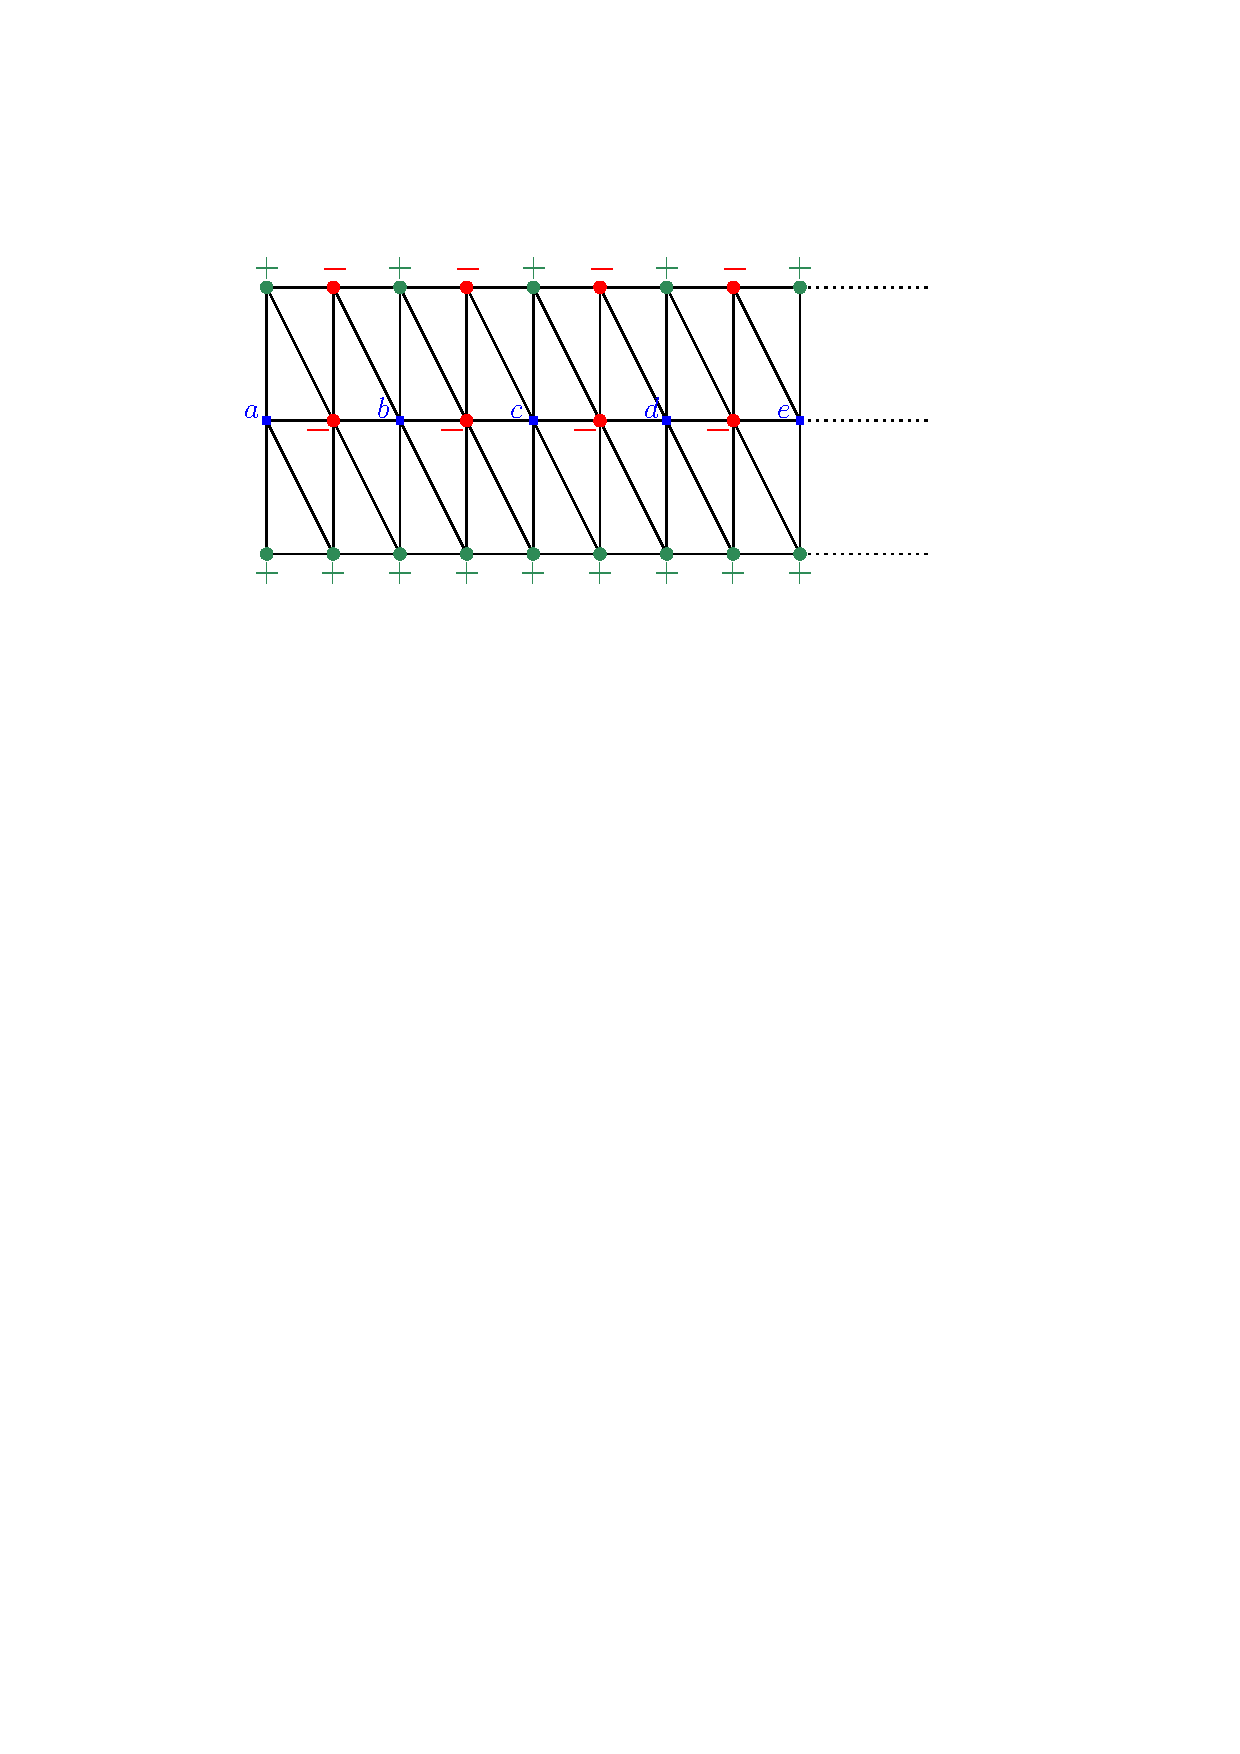
\includegraphics[width=4.0in]{lowerBound}
\end{center}
\vspace{-.2in}
\caption{Reduction from sorting to computing merge trees.}
\figlab{reduction}
\end{figure}
























%\bibliographystyle{alpha}
%\bibliography{connected-components}

\end{document}

